\documentclass[output=paper]{langsci/langscibook}
\ChapterDOI{10.5281/zenodo.3972832}

\author{Jenneke van der Wal\affiliation{Leiden University}}
\title{From macroparameters to microparameters: A Bantu case study}

% \chapterDOI{} %will be filled in at production

\abstract{Crosslinguistic variation in the \ili{Bantu} languages provides evidence
    for a more fine-grained model of parameter setting, ranging from macro- via
    meso- and micro-\is{parameters} to nano-parametric variation, as proposed by
    \citet{BibRob2015}. The various sizes of parametric variation\is{parameters} in
    \ili{Bantu} are discussed for word order, verb movement, ditransitive symmetry,
    locatives, and φ indexing in the clause. Taking a Minimalist
    featural perspective, the resulting emergent parameter settings and
hierarchies are motivated by third-factor principles. The paper furthermore
shows how macrovariation does not equal macroparametric\is{parameters} variation.}

\maketitle

\begin{document}\glsresetall

\section{Parametric variation}\label{bkm:Ref347925115}\label{sec:3.1}

In a Minimalist approach to syntactic variation, the variation is often assumed
to be located in the lexicon, since the items in the lexicon need to be learned
anyway, be they of a lexical or functional nature. This basis of parametric
variation is captured in the \isi{Borer--Chomsky conjecture}
(\citealt[3]{Baker2008}, cf.\ \citealt{Borer1984,Chomsky1995}), building on the
lexical parameterization hypothesis (\citealt{ManziniWexler1987}) and the
functional parameterization hypothesis \citep{Fukui1995}:

\ea All \isi{parameters} of variation are attributable to differences in the features
of particular items (e.g. the functional heads\is{functional items}) in the lexicon.
\z

This entails that parameter settings involve, first, the selection of which
formal features are present in the grammar of a language, and second, where in
the language these features manifest themselves. This creates natural
dependency relations, which can be captured in parameter hierarchies – the
backbone of the ReCoS project as proposed by Ian Roberts (see
\citealt{RobHol2010,Roberts2012} and much work in
collaboration with other members of the project). An example is the hierarchy
for word order \citep{Roberts2012}, assuming that the default is for languages
to be head-initial \citep{Kayne1994} and that head-finality is triggered by a
feature moving the complement to the specifier of the head containing the
feature (see further in \Cref{sub:3.2.1}):

\ea\label{ex:vdwal:3.2} Word order parameter hierarchy\is{parameter hierarchies} \citep{Roberts2012}:
    \begin{tikzpicture}[baseline]

        \Tree 	[.{Is head-final present?}
                    {No: head-initial}
                    [.{Yes: present on all heads?}
                        {Yes: head-final}
                        [.{No: present on [$+$V] heads?}
                            {Yes: head-final\\in the clause only}
                            {No: present on \dots}
                        ]
                    ]
                ]

    \end{tikzpicture}
\z

There are two main conceptual motivations for exploring this hierarchical model
of parameterisation. First, organising \isi{parameters} in a dependency relation
– rather than postulating independent parameters – drastically reduces the number
of possible combinations of parameter settings, i.e. the number of possible
grammars, as shown by \citet{RobHol2010}, \citet{Sheehan2014}, and
\citet{BibHolRob2014}.

Second, the parameter hierarchy\is{parameter hierarchies} can serve to model a path of acquisition\is{language acquisition} that
is shaped by general learning biases (a component of the \enquote{third factor} in
language design, \citealt{Chomsky2005}). \textcite{BibRob2015,BibRob2017}
suggest that two general learning biases combine to form a \enquote{minimax search
algorithm}:

\ea \textcite[300]{BibRob2015}
    \ea \gls{FE}\\
        Postulate as few features as possible to account for the input.
    \ex \gls{IG}\\
        If a functional head\is{functional items} sets a parameter to value v\textsubscript{i} then
        there is a preference for all functional heads\is{functional items} to set this parameter to
        value v\textsubscript{i} \\ (a.k.a. “maximise available features”)
    \z
\z

By \gls{FE}, the first parameter is always whether a feature is
present/gram\-mat\-i\-calised in a language at all (cf.\
\citealt{GiaGuaLon2008}). If there is no evidence for the presence of the
feature, this first question will not even be asked. If there is evidence, a
formal feature is posited, and by \gls{IG} the feature is taken to be present
on all heads. Only if there is counterevidence in the \gls{PLD}\is{primary
linguistic data}\is{PLD|see{primary linguistic data}} for this omnipresence
will an acquirer postulate new categories and ask more specific questions about
the distribution of the feature, i.e. on which subset of heads the feature is
present. We thus derive a \enquote{none-all-some} order of implicational
parameters and of parameter acquisition\is{language acquisition}, as
represented in \eqref{ex:vdwal:3.5}.  Parameters in this system are thus an
emergent property of the grammar; see \textcite{BibRob2015,BibRob2016},
\textcite{Biberauer2017,Biberauer2017c,Biberauer2018} , and
\textcite{Roberts2019} for a full explanation of this emergent parameter
setting.

\begin{exe}
    \ex\label{bkm:Ref347566517}\label{ex:vdwal:3.5}%
    \begin{tikzpicture}[baseline=(F.base)]
        \Tree 	[.\node(F){F present?};
                    {\textsc{no}}
                    [.\node(y){\textsc{yes}:};
                        {\textsc{yes}}
                        \node(n){\textsc{no}:};
                    ]
                ]

        \node [right=3mm of y.center] {all heads?};
        \node [right=3mm of n.center] {which subset of heads?};
    \end{tikzpicture}
\end{exe}

This \textsc{none > all > some} acquisition\is{language acquisition} creates a hierarchy that we can think of as
ever more specified (i.e. featurally rich) \isi{parameters}. In “size” terms,
\textcite{BibRob2015,BibRob2016} propose the following taxonomy of parameters:

\ea\label{ex:vdwal:3.6} Types of parameters\\
    For a given value \emph{v\textsubscript{i}} of a parametrically variant
    feature F:
    \ea Macroparameters: all heads of the relevant type, e.g. all probes, all
    phase\is{phases} heads, share \emph{v\textsubscript{i}};
    \ex Mesoparameters: all heads of a given natural class, e.g. [$+$V] or a core
    functional category, share \emph{v\textsubscript{i}};
    \ex Microparameters: a small, lexically definable subclass of functional
    heads (e.g. modal auxiliaries, subject clitics) share
    \emph{v\textsubscript{i}};
    \ex Nanoparameters: one or more individual lexical items is/are specified
    for \emph{v\textsubscript{i}}.
    \z
\z

These parameter settings are said to have consequences for typology,
acquisition, and diachrony. True macroparameters sit at the top of the
hierarchy, determined by the complete absence or omnipresence of a feature.
Typologically, the subsequent parameter settings have longer and more complex
featural descriptions (since the descriptions are essentially aggregates of
prior parameter settings), indicative of increasingly more marked grammatical
systems. In terms of acquisition\is{language acquisition}, the higher \isi{parameters} need to be set before
lower \isi{parameters} can be, which means that the further down the hierarchy a
parameter is, the further it is expected to be along a learning path.

A conceptual motivation for the various sizes of parametric variation\is{parameters} has thus
been presented in the work by Biberauer and Roberts, but there remains a need
for empirical evidence for these size differences.
\textcite{BibRob2012,BibRob2016} and \citet{Ledgeway2013} form a good start,
and the first goal of the current paper is to show that the different sizes of
parametric variation are empirically verifiable in the \ili{Bantu} languages,
allowing a clearer insight into the nature of cross-Bantu variation, and a
finer-grained discussion of how languages differ parametrically.

\largerpage
A second goal of the current paper is to show how parameter setting sizes need
to be distinguished from geographical and genealogical \enquote{sizes} of variation.
This is an important distinction that is not always made explicit: there is a
difference between \emph{sizes of variation} and \emph{sizes of parameter
settings}. The terms \enquote{macrovariation} and
\enquote{microvariation}\is{microvariation} are standardly used
when referring to comparative differences in a respectively larger or smaller
geographical area, or at a respectively higher or lower level of genealogical
relations. For example, one might talk about macrovariation between Algonquian
vs.\ Sinitic languages (e.g. for polysynthetic vs.\ analytic morphology), or
\isi{microvariation} among northern Italian dialects. Given the relative robustness
and stability of higher \isi{parameters} with respect to lower \isi{parameters}, we expect
the variation in parameter size to go together with this geographical and
genealogical variation. Logically speaking, however, the two are distinct. For
example, if the presence of the feature uCase\is{case!abstract Case} is one of the \isi{parameters}, then it
can be set as a macroparameter: either DPs need to be licensed or they do
not.\footnote{\textcite{Halpert2012,Halpert2016} and
    \citet{CarstensMletshe2015} suggest that even if uCase\is{case!abstract Case} is absent on T (no
    evidence for nominative/subject case),\is{nominative case} there might still be a requirement
    for nominals in the lower domain to be licensed. Halpert claims that bare
    nominals can be Case\is{case!Case licensing} licensed either inherently if they have an augment (K)
    or by a clause head while in the vP domain;
    \citeauthor{CarstensMletshe2015} propose semantic Case
    licensing\is{case!Case licensing} by a low
Focus head along with a value for [Focus].  This suggests a micro setting for
the Case\is{case!abstract Case} parameter in these languages.} \citet{Diercks2012} shows that some
Bantu languages do not show evidence for the presence of
uCase,\is{case!abstract Case} essentially
setting the first parameter in this potential hierarchy to \enquote{no}: uCase\is{case!abstract Case} features
are not present. In contrast, I show that at least the \ili{Bantu} languages \ili{Makhuwa}
and \ili{Matengo} do show evidence for the presence of abstract Case\is{case!abstract Case}
\parencite{vanderWal2015}, which again appears to be set as a macroparameter
for the whole language. This means that we find both macroparametric\is{parameters} settings
(\enquote{no} and \enquote{all}) in different \ili{Bantu} languages.  Although this is a variation in
macroparametric settings, it would not typically be described as
macrovariation, since it concerns variation within a subfamily.

With this background and these aims, the rest of the paper illustrates the
various sizes of parametric variation\is{parameters} across \ili{Bantu}.
\Cref{sec:3.2} exemplifies each parameter size (from macro to nano) from
different domains: word order, \isi{verb movement},\is{head movement} symmetry in
double objects,\is{double object construction} and locatives.  \Cref{sec:3.3} focuses on one domain, φ
feature\is{φ-features} indexing, and attempts to establish a parameter
hierarchy\is{parameter hierarchies}, capturing the variation as found in the
\ili{Bantu} languages, and exploring the nature of parameter hierarchies in the
process.\is{DOC|see{double object construction}}

\section{One size does not fit all: Bantu illustrations of parameter
sizes}\label{sec:3.2}

\subsection{Macro setting: Word order parameter}\label{sub:3.2.1}

Under the assumption that head-initiality is the basic parameter setting
\citep{Kayne1994}, head-finality can be seen as the presence of a
\isi{movement} feature triggering “roll-up” movement.\is{roll-up movement} This
feature can then be present on no heads, all heads, or a subset of heads, as
already referred to above. The \ili{Bantu} languages are almost all straightforwardly
head-initial in all domains: initial complementisers\is{complementizers}, aux-V order, V-O order,
prepositions, and N-possessor order, as illustrated in \eqref{ex:vdwal:3.6}.

\ea\label{bkm:Ref343702566}\ili{Swahili} (G42, Lydia Gilbert, p.c.)\footnote{Bantu languages are classified with a letter (region) and number (language), according to \citegen{Maho2009} update of the original classification by \citet{Guthrie1948}.}\\
    \gll    A-li-ni-ambia  kwamba  a-ta-enda  ku-nunua  mkate bila  mfuko  w-a  wazazi.\\
            \First\Sm{}{}-\Pst-\Fsg{}.\Om{}-tell  \Comp{}  \First\Sm{}-\Fut-go \Inf{}-buy  3.bread without  3.bag  3-\Conn{}  2.parents\\
    \glt    ‘S/he told me that s/he would go to buy bread without her parents’ bag.’
\z

In a parameter hierarchy\is{parameter hierarchies} for word order as in \eqref{ex:vdwal:3.2} above, the \ili{Bantu}
languages overall are in the initial state: no head-final features. In
acquisition this means that the parameter is left as unspecified, since there
is no evidence whatsoever in the \gls{PLD}\is{primary linguistic data} that would trigger an acquirer to even
consider the presence and spread of the feature.

In this case, a macro-setting for the word order parameter happens to also be
associated with macro-variation, in the sense that there is not much variation
\emph{within} the \ili{Bantu} language family but only on a macro-level of comparing
language families.

However, there are tiny patches of head-finality to be found here and there.
Two examples are O-V order in \ili{Tunen}, and final question particles in
languages like \ili{Rangi}\footnote{Rangi (like some surrounding languages) is
    famous for its main clause V-aux order in two future tenses
    \citep{Gibson2016}, which is an instance of head-finality too. However, the
    fact that the object still follows the auxiliary\is{auxiliaries} argues
    against roll-up movement,\is{roll-up movement} and thus against an analysis
    as involving the same feature. Furthermore, the strict adjacency required
    between the infinitival verb and the auxiliary\is{auxiliaries}, as well as
    the fact that clauses with a filled C-domain (relative, cleft,\is{clefts}
    wh, \isi{focus}) require aux-V order,  argues in favour of V-aux as a
derived by phrasal movement\is{movement} of only the infinitive to the
specifier of the aux, rather than a full comp-to-spec movement.} and
\ili{Zulu}.  While these languages are otherwise head-initial, they show
head-finality in some restricted areas of the grammar.

\ili{Tunen} is one of very few \ili{Bantu} languages in which the direct object typically
precedes the verb (\ref{ex:vdwal:3.7}a). Only when the object is (contrastively)
focused\is{focus!contrastive focus} will it follow the verb, and in addition be marked with a contrastive
particle \emph{á} (\ref{ex:vdwal:3.7}b).

\ea\label{bkm:Ref373494395}\label{ex:vdwal:3.7}\ili{Tunen} (A44, \citealt[126]{Mous1997})
    \ea
    \gll 	\`{A}ná  mònɛ  índì.\\
            \Tsg{}.\Pst{}  money  give\\
    \glt    \enquote*{S/he gave money.}
    \ex
    \gll 	\`{A}ná  índì  á  mònɛ.\\
            \Tsg{}.\Pst{}  give  \Ptcl{}  money\\
    \glt    \enquote*{S/he gave MONEY.}
    \z
\z

Final particles form another example: while complementisers\is{complementizers} typically precede
the clause they embed, question particles in \ili{Zulu} and \ili{Rangi} are clearly
clause-final, evidencing a high interrogative-related projection (cf.\
\citealt{Buell2005,Buell2011}).\largerpage[-2]

\ea\label{ex:vdwal:3.8}\ili{Zulu} (S42, \citealt[69]{Buell2005})
	\ea
	\gll	U-Sipho  u-ya-yi-thanda  lo-mculo.\\
            \Aug-1.Sipho  1\Sm-\Dj-9\Om{}-love  3.\Dem{}-3.song\\
	\glt    ‘Sipho likes this song.’
	\ex
	\gll	 U-Sipho  u-ya-yi-thanda  lo-mculo  na?\\
            \Aug-1.Sipho  1\Sm-\Dj-9\Om{}-love  3.\Dem{}-3.song  \glossQ{}\\
	\glt    ‘Does Sipho like this song?’
    \z\pagebreak
\ex \ili{Rangi} (F33, \citealt[51]{Gibson2012})
    \ea
	\gll	 Ma-saare  y-áányu  mwi-ter-iwre  ʉʉ?\\
            6-words  6-your  \Spl.\Sm{}.\Pst{}-listen-\Pfv.\Pass{}  \glossQ{}\\
	\glt    ‘Were your words listened to?’
	\ex
	\gll	 Nɨ  w-arɨ  w-óó-sáák-a  úry-a  wʉʉ?\\
            \Cop{}  14-stiff.porridge  \Ssg.\Sm-\Prog{}-want-\Fv{}  eat-\Fv{}  \glossQ{}\\
    \glt    ‘Is it stiff porridge that you want to eat?’
	\z
\z

While the typical \ili{Bantu} acquirer generally does not pay any attention to the
word order parameter and happily leaves the \enquote{no} setting intact, the
illustrated phenomena provide potential input to the \ili{Rangi} or \ili{Tunen} acquirer
that the \enquote{no} setting is not quite right. It is also clear that not all heads
are head-final (skip macro), and that the verbal domain is not head-final in
its entirety either (skip meso), which means that the head-final feature is at
most only present on a subclass of heads, i.e. a micro-setting. Specifically
for \ili{Tunen}, it seems to only be present on V,\footnote{This is likely a subset
of V that c-selects for a DP object, as for example CP complements still follow
the verb.} and in \ili{Rangi} and \ili{Zulu} only on a head in the high discourse domain of
the clause.

\subsection{Meso setting: Clausal head movement}\label{sub:3.2.2}

Another point where \ili{Bantu} languages do not seem to vary internally is the
template of verbal morphology and the structural position of the verb stem.
Bantu verbs consist of a root with inflectional prefixes and (mostly optional)
derivational suffixes, ordered as in the simplified template in
\Cref{fig:vdwal:1}.\footnote{Some \ili{Bantu} languages also use \gls{TAM} inflections
    suffixes. An anonymous reviewer points out that \gls{TAM} marking in
    \ili{Chimwiini} is prefixal in general, with the exception of the past tense,
    which is a suffix.  Whether this exception is due to a syntactic
nano-parameter or a different morphological specification remains a question
for further research.}\largerpage[-2]

\begin{figure}[H]
    \begin{tikzpicture}
    \matrix [
              matrix of nodes,
              every node/.style={draw, font=\strut, minimum height=2.6\baselineskip},
            ]
      {
        \Neg{} & subject & \Neg{} & \gls{TAM} & object & \textbf{root} &
        \parbox[c]{1.75cm}{\raggedright \Appl{}, \Pass,\linebreak \Caus, etc.} &
        final suffix & post-final\\
       };
    \end{tikzpicture}%
    \caption{Slots in the \ili{Bantu} verb}\label{fig:vdwal:1}
\end{figure}

This verbal morphology provides clear clues as to its underlying syntax. The
most attractive structural analysis of this verbal structure is, following
\citet{Myers1990}, \citet{Julien2002}, \citet{Kinyalolo2003},
\citet{Carstens2005} and \citet{Buell2005}, and drawing on the explanation in
\textcite{vanderWal2009}, that the verb starts out as a root and incorporates
the derivational and inflectional \emph{suf}fixes by \isi{head movement} in the
lower part of the clause.  It then terminates in a position lower than T. The
inflectional \emph{pre}fixes on the verb represent functional heads\is{functional items} spelled out
in their base positions. The (derived) verb stem and prefixes form one word by
phonological merger. See \citet{Julien2002} for the more elaborate
argumentation.\largerpage

To illustrate and argue for this derivation, consider first the \ili{Makhuwa}
example in \eqref{ex:vdwal:3.10} and the proposed derivation in
\eqref{ex:vdwal:3.11}. The verb stem \emph{-oon-} ‘to see’, head-moves to CausP
and incorporates the causative morpheme to its left: \emph{-oon-ih-}. This
combined head moves on to ApplP, incorporating a further suffix to its left:
\emph{-oon-ih-er-}. The next step adds the \isi{passive} morpheme to form
\emph{-oon-ih-er-iy-} and this complex moves once more to add the final suffix,
which has been posited in an aspectual projection just above vP. Crucially,
these are all suffixes, and they surface in reversed order of structural
hierarchy (\citeauthor{Baker1988}'s \citeyear{Baker1988} \isi{mirror
principle}).

\ea\label{ex:vdwal:3.10} \ili{Makhuwa} (P31, \citealt[168--169]{vanderWal2009})\\
    \gll  nlópwáná  o-h-oón-íh-er-íy-á  epuluútsá\\
        1.man  1\Sm-\Pfv{}.\Dj{}-see-\Caus{}-\Appl{}-\Pass{}-\Fv{}  9.blouse\\
    \glt    ‘the man was shown the blouse’
\z

\ea\label{ex:vdwal:3.11}
    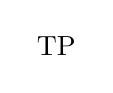
\begin{tikzpicture}[baseline=(T.base)]

        \Tree 	[.\node(T){TP};
                    o-h-
                    [.AspP
                        {[[[[[-oon]\tss{i}ih]\tss{j}er]\tss{k}iy]\tss{m}a]}
                        [.vP
                            {}
                            [.PassP\footnotemark{}
                                t\tss{m}
                                [.ApplP
                                    t\tss{k}
                                    [.CausP
                                        t\tss{j}
                                        [.VP
                                            t\tss{i}
                                            epuluutsa
                                        ]
                                    ]
                                ]
                            ]
                        ]
                    ]
                ]

    \end{tikzpicture}
\z
\footnotetext{The \isi{passive} morpheme can also reside in a higher VoiceP; for the
current point it does not make a difference.}

One might expect the verb to move even higher (v-to-T-to-C), but there is no
reason to assume that a moved head will first incorporate morphemes to its
right (the derivational extensions and final inflectional suffix) and then to
its left (the \isi{agreement} and \gls{TAM} markers). Therefore, the fact that
inflectional morphemes surface as prefixes strongly suggests that these are not
incorporated into the verb in the same way as the derivational suffixes, and
thus that the verb has not head-moved further in the inflectional domain. The
prefixes do form one phonological unit with the verb stem, but are posited as
individual heads that attach to the rest of the verb by phonological merger
only.

Another argument for this analysis is found in the order of the prefixes. If
the inflectional prefixes were also the result of \isi{head movement}, like the
suffixes, they are expected to surface in the opposite order. This is indeed
what we find in \ili{French}, where there is independent evidence that the verb moves
to T: the inflectional morphemes appear in the reverse order of the \ili{Makhuwa}
inflectional prefixes \eqref{ex:vdwal:3.12}, and they appear as suffixes on the verb
in \eqref{ex:vdwal:3.13}.

\ea\label{ex:vdwal:3.12} \il{Makhuwa}Makhuwa (P31, \citealt[169]{vanderWal2009})\\
    \gll kha-mw-aa-tsúwéla\\
        \Neg{}-\Spl.\Sm{}-\Ipfv{}-know\\
    \glt ‘you didn't know’
\ex\label{ex:vdwal:3.13} French\il{French}\\
    \gll  nous  aim-er-i-ons\\
          \Fpl{}.\Pron{}  love-\Irr{}-\Pst{}-\Fsg{}\\
    \glt  ‘we would love’
\z

The verbal morphology thus provides evidence for \isi{head movement} of the
verb in the lower part of the clause to a position just outside of vP, with the
prefixes spelled out in their individual positions in the inflectional domain
above vP/AspP. Assuming with \citet{Roberts2010} that \isi{head movement} is
triggered by features on heads (and a subset relation of the features of the
goal with respect to its probe), then in featural terms, \ili{Bantu} verbal
movement\is{head movement} can be accounted for by the distribution of this
feature in the lower part of the clause only. More precisely: only the heads in
the lower phase\is{phases} trigger head movement, but not the higher phase\is{phases}: a
mesoparametric setting (see also \citealt{Ledgeway2013} and
\citealt{Schifano2015} for a parametric account of variation in height of verb
movement\is{head movement} in \ili{Romance}).

Coming back to the distinction between macrovariation and macroparametric
variation, notice that the vast majority of the language family displays this
“halfway” \isi{head movement}. This is an invariant “macro” fact about \ili{Bantu}
\emph{crosslinguistic} (non-)variation that nevertheless clearly is at a
meso-level of \emph{parametric} variation, illustrating again that these
notions should be kept apart.

\subsection{Micro setting: (A)symmetrical double objects}\label{sub:3.2.3}

Ditransitives in \ili{Bantu} languages show crosslinguistic variation as well as
lan\-guage-internal variation in the behaviour of the two internal arguments.
\citet{BresMosh1990} divided \ili{Bantu} languages into two classes -- symmetrical
and asymmetrical -- based on the behaviour of objects in ditransitives:
languages are taken to be symmetrical if both objects of a ditransitive
verb\is{ditransitive constructions}
behave alike with respect to \isi{object marking} and passivisation (see
\citealt{Ngonyani1996,Buell2005} for further tests). In \ili{Zulu}, for
example, either object can be object-marked on the verb \eqref{ex:vdwal:3.14},
making this a \enquote{symmetrical} language.\footnote{One should, however, be careful
    in characterising a whole language as one type, since it has become more
    and more evident that languages are usually only partly symmetrical
    (\citealt{Schadeberg1995,Rugemalira1991,Thwala2006,Ngonyani1996,NgonyaniGithinji2006,Riedel2009,Baker1988,AlsinaMchombo1993,Simango1995,ZellerNgoboka2006,Jerro2015};
\citealt{vanderWal2017}, etc.).}

\ea\label{ex:vdwal:3.14}Zulu (S42, \citealt[11]{Adams2010})
	\ea
	\gll	 U-mama  u-nik-e  aba-ntwana   in-cwadi.\\
	    1a-mama  1\Sm{}{}-give-\Pfv{}  2-children  9-book\\
	\glt    ‘Mama gave the children a book.’
	\ex
	\gll	 U-mama  u-\textbf{ba}{}-nik-e  in-cwadi  (aba-ntwana).\\
	    1a-mama  1\Sm{}{}-\textbf{2\Om{}}-give-\Pfv{}  9-book  2-children\\
	\glt    ‘Mama gave them a book (the children).’
	\ex
    \gll U-mama  u-\textbf{yi}{}-nik-e  aba-ntwana   (in-cwadi).\\
    1a-mama  1\Sm{}{}-\textbf{9\Om{}}-give-\Pfv{}  2-children  9-book\\
    \glt ‘Mama gave the children it (a book).’
    \z
\z

Conversely, in asymmetrical languages only the highest object (benefactive,
recipient) can be object-marked; object-marking the lower object (theme) is
ungrammatical.

\ea\label{ex:vdwal:3.15} Swahili (G42)
    \ea[]{A-li-\textbf{m}{}-pa kitabu.\\
    ‘She gave him a book.’}
    \ex[*]{A-li-\textbf{ki}{}-pa Juma.\\
    ‘She gave it to Juma.’}
    \z
\z

Following \textcite{HaddicanHolmberg2012,HaddicanHolmberg2015}, I propose in
\textcite{vanderWal2017} that symmetry in \ili{Bantu} languages derives from the
ability of lower functional heads\is{functional items} like the Applicative to (Case)\is{case!Case
licensing} license an
argument either in its complement or in its specifier, as in \eqref{ex:vdwal:3.16}
and \eqref{ex:vdwal:3.17}.\glsunset{BEN}\glsunset{TH}

\ea\label{ex:vdwal:3.16}v agrees with \gls{BEN} (and can spell out as Benefactive object marker)\\
    \vskip-\baselineskip
    \begin{tikzpicture}[baseline]
        \Tree 	[.{}
                    \node (v) {v[φ]};
                    [.ApplP
                        \node (ben) {\gls{BEN}};
                        [.{Appl}
                            \node (appl) {Appl};
                            [.VP
                                V
                                \node (th) {\gls{TH}};
                            ]
                        ]
                    ]
                ]

        \draw [arrow, dashed, bend right] (v.south) to (ben.west);
        \draw [arrow, dashed, bend right=60] (appl.south) to (th.south);
    \end{tikzpicture}
\z

\ea\label{ex:vdwal:3.17}v agrees with \gls{TH} (and can spell out as Theme object marker)\\
    \vskip-\baselineskip
    \begin{tikzpicture}[baseline]
        \Tree 	[.{}
                    \node (v) {v[φ]};
                    [.ApplP
                        \node (ben) {\gls{BEN}};
                        [.{Appl}
                            \node (appl) {Appl};
                            [.VP
                                V
                                \node (th) {\gls{TH}};
                            ]
                        ]
                    ]
                ]

        \draw [arrow, dashed, bend left] (appl.west) to (ben.south);
        \draw [arrow, dashed, bend right=60] (v.south) to (th.south);

    \end{tikzpicture}
\z

In asymmetrical languages, Appl always licenses the theme and \eqref{ex:vdwal:3.16}
is the only possible derivation, whereas in symmetrical languages Appl is
flexible in licensing either argument (and either derivation in \eqref{ex:vdwal:3.16}
and \eqref{ex:vdwal:3.17} is possible). The features involved in flexible licensing
are discussed in \textcite{vanderWal2017}, but for the current discussion it
suffices to take this licensing flexibility to account for the difference
between asymmetrical and symmetrical languages.

However, within these “symmetrical” languages, there is variation in which low
functional heads are flexible. That is, lexical ditransitives\is{ditransitive constructions}, applicative
verbs and causative verbs differ in symmetry, across and within languages. For
example, in \ili{Otjiherero}\il{Herero|see{Otjiherero}} the lexical
ditransitive (not shown) and applied verb \eqref{ex:vdwal:3.19} behave
symmetrically for \isi{object marking}, but causatives are asymmetrical, only
allowing \isi{object marking} of the causee and not the theme \eqref{ex:vdwal:3.20}.

\ea\label{ex:vdwal:3.19}\ili{Otjiherero} (R30, \citealt[247]{MartenKula2012})\\
    Applicative\\
	\ea
	\gll	 Má-vé  \textbf{vè}  tjáng-ér-é  òm-bàpírà.\\
	    \Prs{}-2\Sm{}  2\Om{}  write-\Appl{}{}-\Fv{}  9-letter \\
	\glt    ‘They are writing them a letter.’
	\ex
	\gll	 Má-vá  \textbf{ì}  tjáng-ér-é  òvà-nâtjé.\\
	    \Prs-2\Sm{}  9\Om{}  write-\Appl{}{}-\Fv{}  2-children\\
	\glt    ‘They are writing the children it.’
	\z
\ex\label{ex:vdwal:3.20}\ili{Otjiherero} (R30, Jekura Kavari, personal communication)\\
    Causative\\
	\ea[]{
	\gll	 Ma-ve  \textbf{ve}  tjang-is-a  om-bapira. \\
	    \Prs{}-2\Sm{}  2\Om{}  write-\Caus{}{}-\Fv{}  9-letter\\
	\glt    ‘They make them write a letter.’}
	\ex[*]{
    \gll Ma-ve  \textbf{i}  tjang-is-a  ova-natje.\\
	      \Prs{}-2\Sm{}  9\Om{}  write-\Caus{}{}-\Fv{}  2-children\\
	\glt      ‘They make the children write it.’}
	\z
\z
This means that flexibility is present only in a subset of functional heads\is{functional items} in
the lower phase\is{phases}, i.e.\ a microparameter, and within that subset we can
distinguish even further microparameterisation, for example only applicative
but not causative in \ili{Otjiherero}. Moreover, there appears to be an
implicational relation\is{implicational relations} as to which types of ditransitives\is{ditransitive
constructions} show symmetrical object behaviour \citep{vanderWal2017},
shown in~\Cref{tab:vdwal:1}.

\begin{table}
\begin{tabular}{cccl}
\lsptoprule
\Caus{} & \Appl{} & \textsc{ditrans} & Languages\\
\midrule
\cellcolor{white}\ding{51} & \cellcolor{white}\ding{51} & \cellcolor{white}\ding{51} & Zulu, Shona, Lubukusu, Kîîtharaka, Kimeru\\
\ding{55}                           & \cellcolor{white}\ding{51} & \cellcolor{white}\ding{51} & Otjiherero, Southern Sotho\\
\ding{55}                           & \ding{55}                           & \cellcolor{white}\ding{51} & Luguru\\
\ding{55}                           & \ding{55}                           & \ding{55}                           & Swahili etc. (asymmetrical)\\
\lspbottomrule
\end{tabular}
\caption{Implicational relation in ditransitive symmetry}\label{tab:vdwal:1}
\end{table}

\il{Zulu}\il{Shona}\il{Lubukusu}\il{Kîîtharaka}\il{Kimeru}\il{Otjiherero}
\il{Southern Sotho}\il{Luguru}\il{Swahili}
How can this relation be accounted for? Following \citet{Pylkkanen2008}, I take
the lexical ditransitive to involve a low applicative head (LApplP) under V.
Applicative verbs contain a high applicative head (HApplP) between V and v, and
Causative verbs have a causative head (CausP) above HApplP, either between V
and v or above a second little v (see further \citealt{Pylkkanen2008} on
different heights of causatives). The pattern in \tabref{tab:vdwal:1} can then be
understood as an implicational relation\is{implicational relations} between low argument-introducing heads,
such that if a relatively higher head is flexible (= shows symmetrical object
behaviour), lower heads do so too.

For our \isi{parameters}, this means that within the
microparametric\is{parameters} subset of heads (namely, Case
licensing\is{case!Case licensing}
functional heads in the lower phase\is{phases} of the clause), the none-all-some pattern
introduced above re-appears:

\ea Parameter hierarchy\is{parameter hierarchies} for (a)symmetry in
    ditransitive \isi{alignment} (adapted from \citealt{vanderWal2017})\\
        \begin{tikzpicture}[baseline]

            \Tree 	[.{Are low functional heads\is{functional items} flexible in licensing?}
                        {N\\\tuple{\dots}\footnotemark{}}
                        [.\node(all){Y:};
                            {Y\\1: Zulu etc.}
                            [.\node(appl){N:};
                                {Y\\2: \ili{Southern Sotho},\\
                                \ili{Otjiherero}}
                                {N\\3: \ili{Luguru}}
                            ]
                        ]
                    ]

            \node [right=1.5mm of all.center] {Are all low functional
                heads\dots{}?};
            \node [right=1.5mm of appl.center] {Are all Appl heads\dots{}?};

        \end{tikzpicture}
\z
\footnotetext{This is a theoretical possibility, representing flexible
licensing that is sensitive to other factors.}

This falls out naturally if we acknowledge that the creation of a subset type
results from specifying an additional formal feature. Following the same logic,
the basic questions inspired by \gls{FE} and \gls{IG} apply to these features too: the
feature is only postulated if there is evidence (is it present $\to$ yes:
create subset), it is then assumed to be present in the whole subset
(\emph{all} heads within the subset), and only if there is further evidence
that it is not present for all heads in the subset is a further subset created
(defined by another feature). The scope of the parameter settings is thus
growing smaller and smaller the further down the hierarchy a parameter is, but
the mechanism stays the same. The microparameter for object symmetry
illustrated here applies only to the object domain and can therefore be
considered relatively small -- indeed, it is microparametric\is{parameters} variation ---
which in this case also equals a geographical and genealogical size of
\isi{microvariation}.

\subsection{Nano setting: Locatives}\label{sub:3.2.4}

Coming to the smallest size of parametric variation\is{parameters}, it is important to note
that nanoparameters should be distinguished from what \citet[9]{BibRob2015b}
call “parametric fossils”. Syntactic \isi{parameters}, however limited their scope
might be, still have effects in the syntax rather than just affecting the
morphology (as is the case for example in irregular past tenses that have no
syntactic effect). Such a nano-parametric syntactic parameter setting can be
found in Tswana locatives.

The \ili{Bantu} noun classes include a number of locative classes, most
commonly the classes traditionally numbered 16--17--18 and sometimes 23
\citep{Meeussen1967}.  In \ili{Chichewa}, for example, the class 18 prefix
\emph{mu}- derives a locative DP (with meaning \enquote{inside}) from a noun in
a non-locative class, as shown in
\eqref{ex:vdwal:3.22}.\footnote{\citet{Carstens1997} analyses locative DPs as
    null locative nouns taking a KP complement, of which K agrees with the
    locative and spells out as the locative prefix. The reanalysis to a PP then
    concerns the loss of null locative nouns, leaving the KP/PP. Regardless of
    the precise analysis of locatives (locatives as a nominal derivation by
    means of nP being another possibility – see \citealt{FuchsvanderWal2019}),
the process of change from DP to PP and the relics in this area illustrate a
nanoparametric setting.} The DP status can be seen in the locative’s ability to
control subject agreement\is{agreement!subject agreement} and object
agreement\is{agreement!object agreement} on the verb. However, not all
languages retain locatives as a part of the noun class system, as there is
variation in the categorial status of locatives. In some southern \ili{Bantu}
languages locative DPs have undergone the \enquote{great locative shift}
\citep{Marten2010}, reanalysing the locative prefix as a preposition. Locatives
are thus PPs in these languages, as illustrated for \ili{Zulu} in
\eqref{ex:vdwal:3.23}.\largerpage

\ea\label{ex:vdwal:3.22} \ili{Chichewa} (N31,~\citealt[58]{Bresnan1991}; Ron Simango, p.c.)
	\ea
	\gll	 Ndí-ma-\textbf{ku}{}-kóndá  ku  San José. \\
	    \Fsg.\Sm{}{}-\Prs{}.\Hab-17\Om{}-love  17  San Jose\\
	\glt    ‘I like (it) (in) San José.’%        \citep[58]{Bresnan1991}
	\ex
	\gll	 Mu-nyumba  \textbf{mu}{}-na-yera.\\
	    18-9.house  18\Sm{}-\Pst{}-white\\
	\glt    ‘Inside the house is clean.’%  (Ron Simango, p.c.)
    \sn {}[\tss{DP} [\tss{nP} mu [\tss{NP} nyumba]]
	\z
\ex\label{ex:vdwal:3.23}Zulu (S42, \citealt{Buell2007})\\
        \gll Ku-lezi  zindlu  ku-hlala  abantu  abakhubazekile. \\
         17-10.these  10.houses  \Expl-stay  2.people  2.handicapped\\
        \glt ‘In these houses live handicapped people.’
    \sn {}[\textsubscript{PP} ku\textsubscript{} [\textsubscript{DP} lezi [\textsubscript{NP} zindlu]
\z

\citet{RiedelMarten2012} show that there is a continuum for \ili{Bantu} locatives,
ranging from a fully operative three-way (or more) distinction between the
different locative noun classes, on nouns as well as \isi{agreement} markers, to a
completely reanalysed PP-based locative system and a reduced verbal \isi{agreement}
paradigm (\citealt{DemuthMmusi1997,Creissels2011}). Towards the latter end of
this spectrum is Setswana, where locative noun classes have been lost, leaving
behind some “relics”. Only some prepositions show class 16 or 18 morphology
(\ref{ex:vdwal:3.24}a), and only two nouns are inherently in locative classes
(\ref{ex:vdwal:3.24}b,c).

\ea\label{ex:vdwal:3.24} Tswana (S31, \citealt{Creissels2011})
    \ea class 18 \emph{mo-rago ga} ‘behind’
    \ex class 17 \emph{go-lo} ‘place’
    \ex class 16 \emph{fe-lo} ‘place’
    \z
\z

Crucially, \emph{golo} and \emph{felo} are not just lexicalised locatives that
are otherwise adjusted to fit a system without any formally locative arguments,
but they still trigger true class 17 locative \isi{agreement} on the verb, according
to \citet{Creissels2011}. This is important because it means that there still
is a syntactic parameter to be set, rather than the variation being
“fossilised” and purely lexical.

The fact that this syntactic property is restricted to only two lexical items
makes it of a nano-parametric size. This is a fragile but interesting stage of
a parameter – unless the lexical items are highly frequent, there is little
chance that acquirers of the language will have enough input to be able to pick
it up. This means that either the property will spread through the language and
remain part of the system, or that it disappears, essentially catapulting the
language right to the top of the relevant hierarchy, back to the \enquote{none} setting
(cf. \citealt{BibRob2016}). The Tswana locatives seem to be on their
way out, as \citet[36]{Creissels2011} notes that “Tswana speakers tend to
regularize the situation by using \emph{lefelo} (class 5, plural \emph{mafelo})
instead of \emph{felo} [class 16, JW]”. This effectively reanalyses the noun
class of the last remaining inherently locative nouns, leading to the loss of
the productive noun class.

In summary, I have presented evidence for more fine-grained parametric
distinctions ranging from macro- to nano-parameters from various domains of
Ban\-tu syntax. One of the challenges in the ReCoS research programme is to see
how the different sizes of variation all link up in one hierarchy, which is the
topic of the next section on φ feature\is{φ-features} indexation.

\section{Variation in the distribution of φ features}\label{sec:3.3}

Bantu languages tend to be head-marking in the clause, often displaying subject
and \isi{object marking}, as well as complementiser\is{complementizers} \isi{agreement}, but again there is
cross-Bantu variation. A closer look at this parametric variation\is{parameters} in φ feature
indexation turns out to be interesting, both from an empirical and a conceptual
point of view. An attempt at establishing one parameter hierarchy\is{parameter hierarchies} for uφ
features is shown to be problematic, but problematic in an insightful way.

\subsection{Where we see uφ features}\label{sub:3.3.1}

In the current framework, φ feature\is{φ-features} indexation is taken to be a reflection of
an \isi{Agree} relation between a Probe and a Goal (\citealt{Chomsky2000,Chomsky2001}). In
Probe--Goal \isi{agreement}, a head with an uninterpretable feature (uF), called the
Probe, searches its c-command domain for valuation by the closest constituent
with a matching interpretable feature (iF), the Goal. I assume that subject
marking on the verb indicates the presence of a full uφ feature\is{φ-features} specification
on T, and that \isi{object marking} is due to uφ on little v. I take a hybrid
approach to \isi{object marking} as \isi{Agree} with a \isi{defective goal}
\citep{Roberts2010,Iorio2014,vanderWal2015}, which
entails that all \isi{object marking}, be it pronominal (non-doubling) or grammatical
(doubling), involves a φ probe. The presence of uφ features\is{φ-features} on a higher head
like C results in agreeing complementisers\is{complementizers} or separate relative markers on the
verb (\citealt{Carstens2003,Henderson2011}, among others). Finally,
I propose that the presence of uφ features\is{φ-features} on lower functional heads\is{functional items} such as
Appl and Caus results in multiple object markers, illustrated in the example in
\eqref{ex:vdwal:3.25} and structure in \eqref{ex:vdwal:3.26}.\footnote{I leave to
    one side how the \ili{Kinande} \enquote{linkers}
    \parencite{BakerCollins2006,Schneider-Zioga2015} fit into this model -- it
    might be that there is a separate LinkerP head that has uφ features\is{φ-features} (as
\citealt{BakerCollins2006} propose).} The sets of φ features\is{φ-features} on the heads in
the lower part of the clause are “gathered” by \isi{head movement} of the verb
through the lower part of the derivation (see~\Cref{sub:3.2.2} above).  As φ
features differ from the derivational heads themselves, they are spelled out as
prefixes on the verb (unlike the applicative, causative, \isi{passive}, etc., which
appear as suffixes).

\ea\label{ex:vdwal:3.25} \ili{Luganda} (JE15, \citealt[67, 72]{Ssekiryango2006})\label{bkm:Ref286389666}
    \ea
    \gll Maama  a-wa-dde  \textbf{taata}  ssente.\\
        1.mother  \First\Sm{}-give-\Pfv{}  1.father  10.money\\
    \glt    ‘Mother has given father money.’
    \ex
    \gll Maama  a-zi-\textbf{mu}-wa-dde. \\
        1.mother  \First\Sm{}{}-10\Om{}-1\Om{}-give-\Pfv{} \\
    \glt    ‘Mother has given him it.’
    \z
\ex\label{ex:vdwal:3.26}\label{bkm:Ref347511825}
    \begin{tikzpicture}[baseline=(top.base)]

        \Tree 	[.\node(top){vP};
                    \node (v) {v\\{}[uφ]};
                    [.ApplP
                        \node (ben) {\textbf{\gls{BEN}}};
                        [.{}
                            \node (appl) {Appl\\{}[uφ]};
                            [.VP
                                V
                                \node (th) {\underline{\gls{TH}}};
                            ]
                        ]
                    ]
                ]

        \draw [arrow, bend right=60] (v.south) to (ben.south);
        \draw [arrow, bend right=60] (appl.south) to (th.south);

    \end{tikzpicture}
\z

\subsection{First attempt at a hierarchy}\label{sub:3.3.2}

In setting the uφ \isi{parameters} of a language, what needs to be established is
wheth\-er the language makes use of uφ probes at all, and if so, on which heads
these features are present. One can thus imagine a parameter hierarchy\is{parameter hierarchies} as in
\eqref{ex:vdwal:3.27}, following the now-familiar none--all--some
sequence.

\ea\label{bkm:Ref255201037}\label{ex:vdwal:3.27} Possible uφ feature\is{φ-features} hierarchy 1
(cf.\ \citealt{RobHol2010,Roberts2012,Roberts2014})
    \begin{tikzpicture}[baseline]

        \Tree 	[.{Is uφ present?}
                    {N}
                    [.\node(all){Y:};
                        {Y}
                        [.\node(nom){N:};
                            {Y}
                            [.\node(x){N:};
                                {Y}
                                {\dots}
                            ]
                        ]
                    ]
                ]

        \node [right=1.5mm of all.center] {Is uφ present on all heads?};
        \node [right=1.5mm of nom.center, align=left] {Is uφ present on all nominal
            [$+$N]/\\ clausal [$+$V] heads?};
        \node [right=1.5mm of x.center] {Is uφ present on heads with additional feature
            X?};

    \end{tikzpicture}
\z

The first parameter asks whether uninterpretable φ features\is{φ-features} are present at all
in the language. If the answer is \enquote{no}, this could describe radical pro-drop
languages (\citealt{Saito2007},
\citealt{Roberts2010,Roberts2012,Roberts2014,Roberts2019}), which do
not show any cross-indexing and where this question will thus not even come up
for the language acquirer (sticking to \gls{FE}). In contrast, verbal inflection in
all \ili{Bantu} languages shows at least some indexing, which means that it needs to
be established how pervasive this feature is in each language.

By \gls{IG}, the next parameter sets whether \emph{all} probes have uφ. There
is a question as to which heads are included in \enquote{all probes}; concretely,
should both the nominal and verbal domain be considered? This is not the case
for the null subject hierarchy for φ features\is{φ-features} as proposed by
\citet{RobHol2010}, where only the clausal domain is considered. The
acquisition logic of none-all-some, however, requires that the first
\enquote{all}
setting concerns undifferentiated categories (see
\citealt{Biberauer2011,Biberauer2018}, \citealt{Bazalgette2015}, and
\citealt{BibRob2017} on emergent parameters), which means that the
whole domain – which is eventually split into nominal and verbal – should be
considered at this macro stage. Setting this parameter to \enquote{yes} should result in
agreement not just on C, T, v, and Appl but also P, D, Num, and Poss. While
some \ili{Bantu} languages may come close to the presence of uφ features\is{φ-features} throughout
the language,\footnote{There is a question as to whether \isi{agreement} and concord
involve the same operation – see for example \citet{Giusti2008} for discussion
claiming that they are not.} I do not know of any \ili{Bantu} language showing φ
agreement on prepositions,\footnote{I take the \ili{Bantu} connective \emph{-a} ‘of’
to not be a true preposition \parencite{vandeVelde2013}.} so we need to inspect
subtypes.

One step further down the hierarchy we ask whether uφ is present on a subset of
heads, specifically all heads in the nominal or verbal domain. Since it may be
the case that there is a relevant subset in \emph{both} domains, we can see
this as a split in a third dimension where \isi{parameters} are set for the nominal
domain [$+$N] separately from the verbal domain [$+$V], depending on the input.
Focussing on the clausal domain for the current discussion, once the [$+$V]
subset is identified, by \gls{IG} it is assumed that all heads in the subset, i.e.
all functional heads\is{functional items} in the extended verbal projection, have uφ.

An example of a language where uφ features\is{φ-features} are generalised to occur on all
(clausal) heads is \ili{Ciluba}. \ili{Ciluba} displays multiple \isi{object marking} (i.e. uφ on
v and Appl, in the system as introduced above), as well as subject marking (φ
on T) and agreeing relative complementisers\is{complementizers} (φ on C). Object and
subject marking are illustrated in \eqref{ex:vdwal:3.28}; and \eqref{ex:vdwal:3.29} shows
separate subject marking on the verb and relative \isi{agreement} on the
auxiliary\is{auxiliaries}.

\ea\label{ex:vdwal:3.28} \ili{Ciluba} Kasai (L31, \citealt[87]{Cocchi2000})\label{bkm:Ref345186241}\\
    \gll Mukaji  \textbf{u}{}-\textbf{tshi}{}-\textbf{mu}{}-sumb-il-a.\\
          1.woman  1\Sm-7\Om-1\Om{}-buy-\Appl{}{}-\Fv{}\\
    \glt      `The woman buys it (fruit) for him (the boy).’
\ex\label{ex:vdwal:3.29} \ili{Ciluba} Kasai (L31, \citealt[104]{deKindBostoen2012}) \label{bkm:Ref345186270}
	\ea
	\gll	 maamù  \textbf{u}{}-di  ba-àna  \textbf{bà}{}-ambul-il-a  mikàndà…\\
	    1.mother  1\Rm{}-be  2-child  2\Sm{}-carry-\Appl{}{}-\Fv{}  4-book\\
	\glt    ‘mother, for whom the children are carrying the books…’
	\ex
	\gll	 mi-kàndà  \textbf{ì}{}-dì  ba-àna  \textbf{bà}{}-ambul-il-a  maamù…\\
	    4-book  4\Rm{}-be  2-children  2\Sm{}-carry-\Appl{}{}-\Fv{}  1.mother\\
	\glt    ‘the books which the children are carrying for mother…’
	\z
\z

If not all heads in the clause have uφ, further parameterisation consists of
establishing the next relevant subset where uφ is present. For the \ili{Bantu}
clausal domain, the next largest subset appears to be the argument-licensing
heads: T, v, and Appl/Caus. Sticking with a standard view of Case
licensing\is{case!Case licensing},
this would come down to heads that have
Case in a featural specification.\footnote{However, see the discussion on Case in \sectref{bkm:Ref347925115}
    as well as \citet{Diercks2012} and
    \textcite{vanderWal2015}. Even if abstract \is{case!abstract Case} as we know it does
not play a role which is as influential in many European languages, there is
still reason to believe that a nominal licensing constraint is at play
universally, as we show in \textcite{SheevanderWal2016,SheevanderWal2018}.} In
\ili{Kinyarwanda}, the verb famously displays multiple object marking
\eqref{ex:vdwal:3.30} as well as subject marking, but not complementiser or
relative \isi{agreement} for φ features: the relative clause in
\eqref{ex:vdwal:3.31} is formed by a high tone. This means that uφ is
present on v and Appl, as well as T, but not on C.  \ili{Kinyarwanda} thus sets
the parameter \enquote{Is uφ present on all argument-licensing heads?} to
\enquote{yes}, entailing that there is no uφ on C, since otherwise the language
would have already been done setting its \isi{parameters} at the previous
question, i.e.\ all clausal heads have uφ.

\ea\label{ex:vdwal:3.30}Kinyarwanda (JD61, \citealt[183]{BeauNurRos2004})\label{bkm:Ref317954425}\\
    \begin{tabularx}{\linewidth}{@{}lQ@{}} Umugoré & \textbf{a}{}-ra-na-ha-\textbf{ki}{}-\textbf{zi}{}-\textbf{ba}{}-\textbf{ku}{}-\textbf{n-}someesheesherereza.\\
    1.woman & \First\Sm{}{}-\Dj{}-also-16\Om-7\Om{}-10\Om{}-2\Om-\Ssg.\Om-\Fsg.\Om-read.\Caus{}.\Caus{}.\Appl{}.\Appl{}\\
    \end{tabularx}\\
    \glt    ‘The woman is also making us read it (book, cl.\ 7) with them (glasses,
        cl.\ 10) to you for me there (at the house, cl.\ 16).’
\ex \label{ex:vdwal:3.31}Kinyarwanda (JD61, \citealt[11]{ZellerNgoboka2014})\label{bkm:Ref345185298}
	\ea
	\gll	 U-mu-kózi  a-bar-a  i-bi-tabo.\\
	    \Aug{}{}-1-worker  \First\Sm{}{}-count-\Fv{}  \Aug{}{}-8-book\\
	\glt    ‘The worker counts books.’
	\ex
	\gll	 i-bi-tabo  u-mu-kózi  a-bar-á\\
	    \Aug{}{}-8-books  \Aug{}{}-1-worker  \First\Sm{}{}-count-\Fv{}\\
	\glt    ‘the books that the worker counts’
	\z
\z

For all languages setting this parameter to \enquote{no}, a further subset will be
found, forming the next parameter. Within the argument-licensing heads, the
next question is whether uφ is present on heads in the higher phase\is{phases} (i.e. v and
T but not Appl). If the setting is \enquote{yes}, the language has subject marking and
only a single object marker, as illustrated for \ili{Makhuwa}. \ili{Makhuwa} shows
extremely regular subject marking as well as \isi{object marking} (all and only
objects in classes 1 and 2 are marked, \citealt{vanderWal2009}), but is
restricted to one object marker \eqref{ex:vdwal:3.32}, which means φ on T and v, but
not on Appl.

\ea\label{ex:vdwal:3.32} \ili{Makhuwa} (P31) \label{bkm:Ref347928062}\\
    \gll    Xaviéré  \textbf{o}{}-nú-\textbf{ḿ}{}-váhá  anelá  Lusiána.\\
            1.Xavier  1\Sm-\Pfv.\Prs-1\Om{}-give  1.ring  1.Lusiana\\
    \glt        ‘Xavier gave Lusiana a ring.’
\z

\ili{Makhuwa} equally does not show \isi{agreement} on C: complementisers\is{complementizers} never agree, and
the relative construction in \ili{Makhuwa} does not have a relative complementiser\is{complementizers} or
relative \isi{agreement}. Instead, it is best analysed as a nomino-verbal participial
construction which does not have an agreeing C head
\citep{vanderWal2010}.\footnote{What seems to be a subject marker or
relative marker on the relative verb in \ili{Makhuwa} (\emph{e-} and \emph{tsi-} in
the examples) is a pronominal head (PtcpP) coreferring to the referent
indicated by the head noun, e.g. both refer to a class 9 shirt and therefore
are both in class 9. There is no regular subject marking, but the subject can
be pronominalised on the verb as a possessive (-\emph{aawe}), showing that the
relative clause is not a full clause but lacks higher heads in the extended
verbal projection. See \textcite{vanderWal2010} for details.}

\ea \ili{Makhuwa} (P31, \citealt[210]{vanderWal2010})\\
    \gll Ki-m-phéélá  ekanetá  tsi-ki-vah-aly-ááwé  (Alí).\\
        \Fsg-\Sm-\Prs.\Cj-want  10.pens  10-\Fsg.\Om{}-give-\Pfv.\Rel{}-\Poss{}.1  1.Ali\\
    \glt    ‘I want the pens that he (Ali) gave me.’
\z

If the parameter setting is \enquote{no} for the presence of uφ features\is{φ-features} in the higher
phase, then the language only has uφ on one head. This turns out to always be
the highest in the subset left: uφ on T, i.e. only subject marking (see
\Cref{sub:3.3.3} below on the implicational relation\is{implicational relations} for uφ on clausal heads).
\ili{Basaa} illustrates this parameter setting: it has a subject marker, which is
written separately but is obligatory even in the presence of a full DP subject
\eqref{ex:vdwal:3.34}.

\ea\label{ex:vdwal:3.34}Basaa (A43, \citealt[277]{Hyman2003}) \label{bkm:Ref347562219}\\
    \gll    Liwándá  jêm  \textbf{lí}  m  \textsuperscript{!}ɓéná  jɛ  bíjɛk  í  \textsuperscript{!}ndáp.\\
        friend  my  \Sm{}  \Prs{}  do-often  eat  food  in  house\\
    \glt    ‘My friend often eats food in the house.’
\z

Objects, however, are not marked on the verb, and when the object is
pronominalised it simply appears as an independent pronoun following the verb
(\ref{ex:vdwal:3.35}b).

\ea\label{ex:vdwal:3.35} \ili{Basaa} (A43, \citealt[278]{Hyman2003})\label{bkm:Ref347562250}
    \ea
    \gll A  bí  nuŋúl  lítám.\\
        \Sm{}  \Ppp{}  sell  fruit  \\
    \glt    ‘He sold a fruit.’
    \ex A  bí  nuŋúl  jɔ.\\
        ‘He sold it.’
    \z
\z

Finally, \isi{relative clauses} in \ili{Basaa} can be marked with a demonstrative\is{demonstratives}
(\emph{nu} in (\ref{ex:vdwal:3.36}a) and \emph{hi} in (\ref{ex:vdwal:3.36}b), but
\citet{JenksEtAl2017} argue that this is not a C head.

\ea\label{ex:vdwal:3.36} \ili{Basaa} (A43, \citealt[19, 20]{JenksEtAl2017}) \label{bkm:Ref347562274}
    \ea
    \gll    í-mut  (nú)  a  bí  \ds{}jɛ  bíjɛk\\
            \Aug{}{}-1.person  1.\Rel/\Dem{}  1.\Sm{}  \Ppp{}  eat  8.food\\
    \glt        ‘the person that ate the food’
    \ex\label{bkm:Ref347929302}
    \gll    hínuní  (hí)  liwándá  lí  bí  \ds{}tɛhɛ\\
            \Aug{}.19.bird  19.\Rel/\Dem{}  5.friend  5\Sm{}  \Ppp{}  see\\
    \glt        ‘the bird that the friend saw’
    \z
\z

If \citet{JenksEtAl2017} are correct in their analysis of the relative
construction, then \ili{Basaa} can be taken to illustrate a language in which
only T has uφ features\is{φ-features}, whereas C, v and Appl do not.

The parameter hierarchy\is{parameter hierarchies} for \ili{Bantu} languages
discussed so far would thus come out as follows:\largerpage

\ea Possible uφ feature\is{φ-features} hierarchy 2 (to be adjusted)
    \begin{tikzpicture}[baseline]

        \Tree 	[.{Is uφ present?}
                    {N}
                    [.\node(all){Y:};
                        {Y}
                        [.\node(nom){N:};
                            {Y\\\ili{Ciluba}}
                            [.\node(x){N:};
                                {Y\\Kinyarwanda}
                                [.\node(ph){N:};
                                    {Y\\Makhuwa}
                                    {N\\Basaa}
                                ]
                            ]
                        ]
                    ]
                ]

        \node [right=1.5mm of all.center] {Is uφ present on all heads?};
        \node [right=1.5mm of nom.center, align=left] {Is uφ present on all nominal/clausal heads?};
        \node [right=1.5mm of x.center, align=left] {Is uφ present on all\\argument-licensing heads?};
        \node [right=1.5mm of ph.center, align=left] {Is uφ present on\\higher phase\is{phases} (v$+$T)?};

    \end{tikzpicture}
\z

\subsection{(In)dependent parameters}\label{sub:3.3.3}

If this parameter hierarchy\is{parameter hierarchies} represents the typological picture, then it holds
an implicational prediction such that if a language has uφ on one head in the
following scale, it will have uφ on all the heads to its right (as noted for
subject\is{agreement!subject agreement} and object
agreement\is{agreement!object agreement} by \citealt{Moravcsik1974}, cf.\
\citealt{Givon1976,Bobaljik2008}):

\ea\label{ex:vdwal:3.38}
    \gll    C > Appl > v > T\\
    {comp/rel agr} > {multiple OM} > OM > SM\\
\z

Considering the sequence of heads in the verbal extended projection, it is
clear that C is not in the expected position on this implicational hierarchy.
And there are more indications that C is not quite in place in this hierarchy.
For one thing, the evidence for the absence of uφ features\is{φ-features} on C in \ili{Makhuwa} and
\ili{Basaa} is very much dependent on the theoretical analysis of \isi{relative clauses},
which makes the argument for the absence of uφ on C in these languages less
strong. Moreover, there is clear evidence from other \ili{Bantu} languages that φ
agreement on C must be independent of uφ on the argument-licensing heads. This
is illustrated by \ili{Bembe}, which shows the typical \ili{Bantu} subject and object
marking (40b, uφ on T and v), but does not allow more than one object marker
(40c, no uφ on Appl). Non-subject \isi{relative clauses} in \ili{Bembe} can display a
relative marker in addition to a pronominal subject marker \eqref{ex:vdwal:3.41},
indicating that T and C both have their own set of uφ features\is{φ-features}.

\ea\label{ex:vdwal:3.39} \ili{Bembe} (D54, \citealt[103]{Iorio2014}) \label{bkm:Ref298742208}
	\ea[]{\label{ex:vdwal:3.39a}
	\gll	 Twa-h-ile  batu  bokyo.\\
	    \Fpl.\Sm{}-give-\Pst{}  2.people  14.money\\
	\glt    ‘We gave people money.’}
	\ex[]{\label{ex:vdwal:3.39b}
	\gll	 Twa-bo-h-ile  batu.\\
	    \Fpl.\Sm{}-14\Om{}{}-give-\Pst{}  2.people\\
	\glt    ‘We gave it to people.’}
    \ex[*]{\label{ex:vdwal:3.39c}
    \gll Twa-bo-ba-h-ile {/ } \llap{*}Twa-ba-bo-h-ile\\
        \Fpl.\Sm{}-14\Om{}-2\Om{}{}-give-\Pst{} {} \Fpl.\Sm{}-2\Om{}-14\Om{}{}-give-\Pst{}\\
    \glt    intended: ‘We gave them it.’}
	\z
\ex \label{ex:vdwal:3.40} \ili{Bembe} (D54, \citealt[152]{Iorio2014}) \label{bkm:Ref347515914}
	\ea\label{ex:vdwal:3.40a}
	\gll	 Baana  ba-twa-mon-ilé  ba-b-ile  babembe.\\
	    2.children  2\Rm{}-\Fpl.\Sm{}-see-\Pst{}  2\Sm-\Cop-\Pst{}  2.Bembe\\
	\glt    ‘The children whom we saw were \ili{Bembe}.’
	\ex\label{ex:vdwal:3.40b}
	\gll	 bilewa  bi-ba-koch-ilé\\
	    8.food  8\Rm{}-2\Sm{}-buy-\Pst{}\\
	\glt    ‘the food that they bought’
	\z
\z

This cross-linguistic situation, as illustrated in~\Cref{tab:vdwal:2}, suggests
that the presence of uφ features\is{φ-features} on C does not form part of the implicational
hierarchy that holds between the argument-licensing heads T, v and Appl, which
in turn suggests that uφ on C is a parameter that is independent of the
parameter hierarchy for uφ features\is{φ-features}. See also \textcite{Biberauer2017} and
references cited therein on how C behaves differently from lower heads in the
domain of word order as well.

\begin{table}
\begin{tabular}{ *{4}{>{\centering}p{\widthof{Appl}}} l}
\lsptoprule
C                           & T                           & v                           & Appl                        & Example language\\
\midrule
\cellcolor{white}\ding{51} & \cellcolor{white}\ding{51} & \cellcolor{white}\ding{51} & \cellcolor{white}\ding{51} & \ili{Ciluba}\\
                                   & \cellcolor{white}\ding{51} & \cellcolor{white}\ding{51} & \cellcolor{white}\ding{51} & \ili{Kinyarwanda}\\
                                   & \cellcolor{white}\ding{51} & \cellcolor{white}\ding{51} &                                    & \ili{Makhuwa}\\
                                   & \cellcolor{white}\ding{51} &                                    &                                    & \ili{Basaa}\\
\cellcolor{white}\ding{51} & \cellcolor{white}\ding{51} & \cellcolor{white}\ding{51} &                                    & \ili{Bembe}\\
\lspbottomrule
\end{tabular}
\caption{Implicational relation in uφ features\label{tab:vdwal:2}}
\end{table}

However, the implicational hierarchy \emph{does} appear to hold for the
argument-licensing heads: if a language has uφ on Appl (multiple object
marking) then it has uφ on v (single object marking), and if a language has uφ
on v (object marking) then it has uφ on T (subject marking):

\ea\label{ex:vdwal:3.41}
    \gll    Appl  >  v  >  T\\
            {multiple OM}  >  OM  >  SM\\
\z

It is known that v’s Case-assigning\is{case!Case assignment} capacity can be dependent on T’s
(\citealt{Marantz1991,Baker2015}), and it is clear from the data surveyed here
that the same holds for head-marking \isi{agreement} (see \citealt{Roberts2014} on
the same conclusion for \ili{Romance}; and see, among others,
\citealt{Bobaljik2008,Barany2015} for discussion on \isi{implicational
relations}
between heads in the domains of Case\is{case!abstract Case} and
\isi{agreement}).\is{agreement|seealso{object marking}}
Additionally, based on the data surveyed for \ili{Bantu} languages, this
implicational relation\is{implicational relations} can be extended to the lower
functional heads such as Appl. The fact that these implications hold indicates
that argument-licensing heads are a natural class, with a strong relation to φ
feature\is{φ-features} \isi{agreement}.

This suggests a revision of the parameter hierarchy\is{parameter hierarchies} that brings out the
interdependence of argument-licensing heads, keeping C apart. In fact, it
suggests that variation in the presence of uφ features\is{φ-features} on C is a parameter that
is not actually part of this hierarchy, since hierarchies are only attractive
for modelling \emph{dependent} \isi{parameters} (as argued in the original ReCoS
research proposal, see also \citealt{RobHol2010} and \citealt{Sheehan2014}).
The separate \isi{parameters} can then can be modelled as in \eqref{ex:vdwal:3.43},
representing only the dependent \isi{parameters} in a macro-to-micro
hierarchy:%\newpage

\ea\label{ex:vdwal:3.43} \label{bkm:Ref373481316}
    Dependent and independent uφ feature\is{φ-features} \isi{parameters}\\
    \begin{tikzpicture}[baseline]

        \Tree 	[.{Is uφ present?}
                    {N}
                    [.\node(all){Y:};
                        {Y}
                        [.\node(nom){N:};
                            {Y\\\ili{Ciluba}}
                            [.\node(x){N:};
                                {Y\\Kinyarwanda}
                                [.\node(ph){N:};
                                    {Y\\\ili{Makhuwa}}
                                    {N\\\ili{Basaa}}
                                ]
                            ]
                        ]
                    ]
                ]

        \node [right=1.5mm of all.center] {Is uφ present on all heads?};
        \node [right=1.5mm of nom.center, align=left] {Is uφ present on all nominal/clausal heads?};
        \node [right=1.5mm of x.center, align=left] {Is uφ present on all\\argument-licensing heads?};
        \node [right=1.5mm of ph.center, align=left] {Is uφ present on\\higher phase\is{phases} (v$+$T)?};

    %\end{tikzpicture}
    %\begin{tikzpicture}[baseline=-.79\baselineskip]

        \begin{scope}[xshift=0cm, yshift=-5.25cm]
        \Tree   [.{Is uφ present on C?}
                    {N\\Kinyarwanda}
                    {Y\\\ili{Ciluba}}
                ]
        \end{scope}

    \end{tikzpicture}
\z

\subsection{Further subsets}\label{sub:3.3.4}

Potential nanoparametric\is{parameters} variation can also be attested in this domain, as
exemplified by \ili{Luguru} and \ili{Nyakyusa}. These languages do display \isi{object marking},
but only for some predicates. To illustrate with one example: in \ili{Luguru} the
verb \emph{-bona} ‘to see’ requires an object marker and cannot be
grammatically used without it, as shown for \is{animacy}animate and inanimate objects in
\eqref{ex:vdwal:3.44} and \eqref{ex:vdwal:3.45}. The semantically similar verb \emph{-lola}
‘to see/look at’, on the other hand, does not have this requirement and occurs
without object marker \eqref{ex:vdwal:3.46}.

\ea\label{ex:vdwal:3.44} \ili{Luguru} (G35, \citealt[264--265]{MartenRamadhani2001})
    \ea[]{ \label{bkm:Ref347659654}
	\gll	 Ni-w-on-a  iwana.\\
	        \Fsg.\Sm{}.\Tns-2\Om{}{}-see-\Fv{}  2.children\\
	\glt        ‘I saw the children.’}
	\ex[*]{
    \gll	 Ni-on-a  iwana.\\
	        \Fsg.\Sm.\Tns{}{}-see-\Fv{}  2.children\\
	\glt        intended: ‘I saw the children.’}
	\z
\ex\label{ex:vdwal:3.45} \ili{Luguru} (G35, \citealt[264--265]{MartenRamadhani2001})
	\ea[]{\label{bkm:Ref347659657}
	\gll	 Wa-ch-on-a  ichitabu.\\
	    2\Sm{}.\Tns{}-7\Om{}{}-see-\Fv{}  7.book\\
	\glt    ‘They saw the book.’}
	\ex[*]{
    \gll	 Wa-on-a  ichitabu.\\
	    2\Sm{}.\Tns{}{}-see-\Fv{}  7.book\\
	\glt    int. ‘They saw the book.’}
	\z
\ex\label{ex:vdwal:3.46} \ili{Luguru} (G35, \citealt[264--265]{MartenRamadhani2001}) \label{bkm:Ref347659685}\\
    \gll No-bam-aa  ku-lola  iwanu.\\
    \Fsg.\Sm.\Tns{}{}-want-\Fv{}  15-look.at  2.people\\
    \glt ‘I want to look at people.’
\z

\citet{MartenRamadhani2001} claim that this variation in predicates that do or
do not require/allow \isi{object marking} is not due to transitivity or the choice of
object but individual predicates. Nevertheless, it seems that it can be modeled
as variation in v’s selection of a predicate taking an argument instead of an
adjunct, i.e.\ \isi{microvariation}. This would fit the difference between ‘see X’
(argument) and ‘look at X’ (non-argument). What is particularly suggestive in
this case is the fact that the presence of an object marker can influence the
interpretation of a predicate in \ili{Luguru}. Marten and Ramadhani illustrate this
with the predicate -\emph{pfika,} which is usually interpreted as ‘find, meet’
when used with an object marker (\ref{ex:vdwal:3.47}a), but as ‘arrive’ when there
is no object marker (\ref{ex:vdwal:3.47}b).

\ea\label{ex:vdwal:3.47} \ili{Luguru} (G35, \citealt[265--266]{MartenRamadhani2001})
    \ea[]{ \label{bkm:Ref347659728}
	\gll	 Wanzehe  wa-pfi-pfika  ipfitabu.\\
	    2.elders  2\Sm{}.\Tns{}-8\Om{}{}-find  8.books\\
	\glt    ‘The elders found books.’}
	\ex[]{
	\gll	 Wa-pfika  ukaye  kwake.\\
	    2\Sm{}-find  house  \Poss{}\\
	\glt    ‘They have arrived at / been to his home.’}
    \ex[?]{
    \gll    Wanzehe  wa-pfika  ipfitabu.\\
            2.elders  2\Sm{}-find  8.books\\
    \glt        ‘The elders arrived at the books’\\
            intended: ‘The elders found books.’}
    \z
\z

Such a microparametric\is{parameters} account seems less likely for \ili{Nyakyusa} (M31),
which has similar restrictions on \isi{object marking} \citep{Lusekelo2012}. Here
too, the presence of uφ on v is not set for \emph{all} v heads, and transitive
predicates are in one of three groups according to their object marking
abilities/possibilities (Amani \citealt{Lusekelo2012} and p.c.):

\begin{itemize}
    \item impossible (‘cook’, ‘weave’),
    \item obligatory (‘see’, ‘love/like’),
    \item optional (‘smear’, ‘hold/touch’, ‘take’);
\end{itemize}

The first type of predicate never shows \isi{object marking} and thus never projects
a v with uφ features\is{φ-features}. In the second and third type of predicate uφ features
must\slash can be present on v. It is unclear, however, how type 1 can be
distinguished (featurally) from the other two types, or, in other words, how
type 1 forms a natural subset. \isi{object marking} in \ili{Nyakyusa} therefore appears to
be an instance of nanoparametric\is{parameters} variation: individual predicates have/do not
have uφ features\is{φ-features} on v.

What underlies the distinction between the second and third type is equally
unclear; alternatives suggested by anonymous reviewers include a potential
semantic difference for psych vs.\ touch/motion verbs, and a phonological
factor where the initial consonant of the verb stem or syllable structure might
play a role in requiring \isi{object marking}. However, at the moment this is
only speculative and has to await further research on \ili{Nyakyusa}
\isi{object marking}.

Even if the exact size of the parameter setting or the precise features
involved are as yet unknown, it is clear that these languages distinguish
different predicates, that is, different subtypes of little v, when it comes to
the distribution of uφ features\is{φ-features}.\footnote{Note that
    \textcite{Sheehan2014,Sheehan2017} proposes quite extensive subhierarchies
    for little v with respect to ergative alignment,\is{ergative alignment} but
    starting from a different logic underlying the shape of the parameter
hierarchy.} We thus need a further specification of subsets, arriving at the
nano-level where certain predicates have a positive setting for the presence of
φ features\is{φ-features} on v, indicated as v\textsubscript{α} in the adjusted
hierarchy in \eqref{ex:vdwal:3.48}.\footnote{An alternative way of organising the
    hierarchy to make the typological implication fall out would be the
    following sequence of \isi{parameters} (see also \citealt{Barany2015}): Is
    uφ present? > Is uφ present on T? > Is uφ present on v? > Is uφ present on
    Appl? Note, though, that this cannot capture the acquisitional\is{language
    acquisition} path, and hence loses the motivation in the general cognitive
    principles of \gls{FE} and \gls{IG}.}

\ea\label{ex:vdwal:3.48}\label{bkm:Ref348109619}%\vspace{-1\baselineskip}
    \begin{tikzpicture}[baseline=(root.base),scale=.9]
        \Tree 	[.\node(root){Is uφ present?};
                    {N}
                    [.\node(all){Y:};
                        {Y}
                        [.\node(nom){N:};
                            {Y\\Ciluba,\\Kinyarwanda}
                            [.\node(x){N:};
                                {Y\\Makhuwa,\\Bembe}
                                [.\node(ph){N:};
                                    {Y\\Nyakyusa}
                                    {N\\Basaa}
                                ]
                            ]
                        ]
                    ]
                ]

        \node [right=1.5mm of all.center, font=\small] {Is uφ present on all heads?};
        \node [right=1.5mm of nom.center, align=left, font=\small] {Is uφ present on all\\
            \quad{} argument-licensing heads?};
        \node [right=1.5mm of x.center, align=left, font=\small] {Is uφ present on all v\&T?};
        \node [right=1.5mm of ph.center, align=left, font=\small] {Is uφ present on v\tss{α}?};

        \node (bracket) [right=7cm of all, anchor=south west] {$\Bigg\}$};
        \node (macro) [right=.25cm of bracket.center, font=\small] {macro};
        \node at (nom -| macro.west) [align=left, anchor=west, font=\small] {meso};
        \node at (x -| macro.west) [align=left, anchor=west, font=\small] {micro};
        \node at (ph -| macro.west) [align=left, anchor=west, font=\small] {nano};

    \end{tikzpicture}
    \begin{tikzpicture}[baseline, scale=.9]

        \Tree   [.{Is uφ present on C?}
                    {N\\Kinyarwanda, \ili{Bembe}}
                    {Y\\Ciluba, \ili{Makhuwa}}
                ]

    \end{tikzpicture}
\z

This exploration of the hierarchy for uφ \isi{parameters} has thus brought to
light that what is thought to be the same phenomenon in the first instance
might actually not be part of the same parameter hierarchy\is{parameter
hierarchies} -- concretely, the parameter for φ features\is{φ-features} on C was shown to be
set independently of the other heads in the clause. The data also revealed an
interesting implicational relation\is{implicational relations} for φ features\is{φ-features} on argument-licensing heads,
which can be captured in a parameter hierarchy\is{parameter hierarchies} that
considers smaller and smaller subsets representing Bantu-internal\il{Bantu}
parametric variation\is{parameters} from the meso to the nano level.

\section{Conclusions}\label{sec:3.4}

The different sizes of variation as proposed by \citet{BibRob2015}, ranging
from macro to nano, fit the morphosyntactic variation in the \ili{Bantu} languages
better than a simple \enquote{macro} or \enquote{micro}. Importantly, this perspective
encourages us to look seriously at syntactic variation from a featural
perspective. The featural perspective is attractive with the Minimalist
programme in mind, locating parametric variation\is{parameters} in the features (on functional
heads) in the lexicon. With the outlined parameter-setting algorithm motivated
by third-factor principles (\citealt{Biberauer2017,Biberauer2017c};
\citealt{BibRob2017}) we have a promising model accounting for
crosslinguistic variation.

Bantu-internal variation shows that all parameter types are actually attested,
and individual languages vary as to the “grain” of their settings: what is
micro in one system could be nano in another, etc. This is predicted in the
current approach: the “same” phenomenon surfaces in different sizes in
different systems (cf.\ \citealt{BibRob2016,Ledgeway2013}).

The \ili{Bantu} variation also illustrates that the setting of a parameter to a
certain size does not necessarily correspond to geographical or genealogical
macrovariation or microvariation. Whether languages or language families differ
markedly from each other or not (macrovariation) or are more similar but show
variable properties (microvariation) tends to go hand in hand with the size of
the parameter setting (because of diachronic stability), but there is no
one-to-one relation: a language can have a macro setting on a certain parameter
hierarchy where the rest of the family has smaller settings, and the variation
between otherwise similar languages can still be characterised as
microvariation – as is the case for \ili{Bantu}.

The crosslinguistic variation as seen in this paper thus stems from 1. whether
a feature is present in a language at all; 2. on which (subset of) heads the
feature is present; 3. the combination/interaction of different parameter
settings. The current state of research focuses primarily on the first and
second determinants, which necessarily precede the third aspect. Future
research will hopefully shine light on the interaction of the various
parameters and parameter hierarchies, especially since the \enquote{some} options in
any hierarchy are formed by the interaction with features that potentially are
part of their own separate hierarchy. This, however, requires further
conceptual and empirical investigation.

\printchapterglossary{}

\noindent Numbers refer to noun classes, or to persons when followed by \Sg{}
or \Pl{}.  High tones are marked by an acute accent, low tones are unmarked or
marked by a grave accent.

\section*{Acknowledgements}

This research was funded by the European Research Council advanced grant no.\
269752 \enquote{Rethinking comparative syntax}. I am grateful to the members of
the ReCoS team and especially Theresa Biberauer with whom this little project
was started, and furthermore to the helpful comments of three anonymous
reviewers.  Any errors and misrepresentations are mine only.

{\sloppy\printbibliography[heading=subbibliography,notkeyword=this]}

\end{document}
